\section{Design and Implementation}
\begin{figure}[!t]
\centering
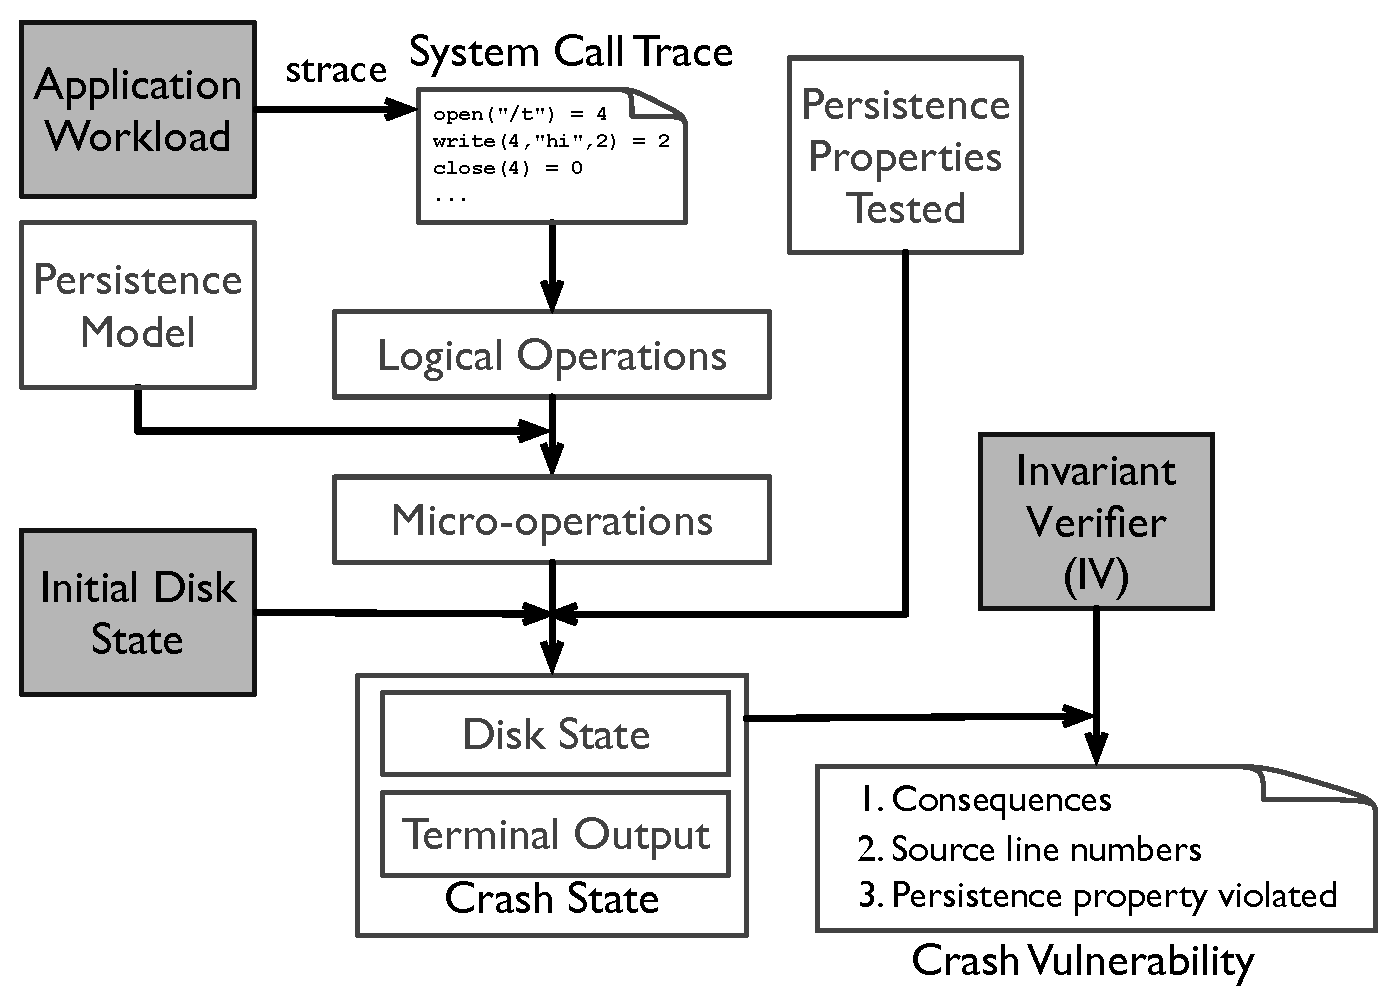
\includegraphics[scale=0.28]{figs/overview2.eps}
\mycaption{fig-overview}{Detecting Vulnerabilities using \toolname}{\footnotesize The
figure shows an overview of how \toolname\ converts user inputs into crash states and
finally into crash vulnerabilities. The shaded grey boxes are inputs supplied by the user.}
\end{figure}



In this section, we explain the design and implementation of \toolname, a
framework to help understand application update protocols, find crash
vulnerabilities in applications, and evaluate the effect of file-system designs
on application-level consistency. 

\subsection{Goals}
\toolname\ is \textit{sound}: every reported vulnerability can be associated with a
crash state possible on the given file-system model. The vulnerability can be
related back to application source code, thus allowing the user to directly
understand problems with the update protocol (\sref{sec-vul-study}). 

\toolname\ requires no changes to the operating system, and runs entirely in
user-space. The file-system model used in \toolname\ can be modified to model
a specific file system, and even new file system designs that have not been
implemented yet (\sref{sec-fs-what-if}). 

\if 0
Our approach can be summed up in one sentence: \textit{find crash states on
which application invariants fail}. Figure~\ref{fig-overview} presents an
overview of the system.

Since we don't know a priori which disk states cause application invariants to
fail, we need a way to systematically explore different possible states
for an application workload. We do this by collecting the system-call trace of
the workload and using an \textit{abstract file-system model}, which defines
what crash states are possible, to generate crash states (\sref{sec-diskstate}).

Even for a simple update protocol, the number of crash states that can be
generated is large enough to rule out exhaustively exploring all crash states.
We use a number of heuristics to selectively explore parts of the space of
crash states (\sref{sec-explore}). 

Given a crash state, we need to know if application invariants fail on that
crash state. We do this by \textit{running the application itself} on top of
each crash state, and inspecting the application state to see if any invariants
have failed (\sref{sec-checker}). Finally, we briefly describe the
implementation of \toolname\ (\sref{sec-implementation}) and discuss its
limitations (\sref{sec-discuss}).  
% Also Overview?
% This is where you explain how one can go from stream of fs syscalls +
% properties to understanding the behavior
\fi

\subsection{Generating Crash States}
\label{sec-diskstate}
To generate crash states, the user supplies the application workload and an
initial disk state. \toolname\ uses \smalltt{strace} to capture the system call
trace of the workload during its execution. The problem then becomes one of
generating crash states given the update protocol in the form of system calls.

The same update protocol can lead to different crash states on different file
systems. Therefore, a file-system model is needed to define the crash states
that are produced by \toolname. Because \toolname\ aims to find vulnerabilities
across all file systems, it uses a file-system model based on an abstract file
system that produces a superset of all the crash states produced by modern file
systems (\sref{sec-model}). 

Some system calls are not atomic in our file-system model. Hence, partial
execution of a system call can lead to a number of \textit{intermediate}
states. For example, consider appending a block to a file. One intermediate
state would be the case where a new block was allocated to the file, and the
file inode is updated, but the block itself is not. Thus the block would
reflect the contents of its previous owner. We would like to capture
intermediate states like these in our model. We break up system calls into
atomic operations called \textit{micro-code} to accomplish this
(\sref{sec-micro-code}). 

We illustrate the concepts of the file-system
model and micro-code with an example (\sref{sec-example}). Finally, we explain
how the crash state is generated (\sref{sec-construct}). 

%\begin{lstlisting}[float=t, caption = {\textbf{System call trace for a toy
update protocol}. {\em \small The protocol writes a file, syncs it, writes the
file again, and links it a new location. Finally it records the operation as
done on stdout.} }, label = {lst-syscall}, escapechar=!]

1 open(pathname="/x2VC") = 10
2 pwrite(fd=10, offset=0, data="foo", size=3)
3 fsync(fd=10)
4 pwrite(fd=10, offset=3, data="bar", size=3)
5 link(oldpath="/x2VC", newpath="/file")
6 pwrite(fd=1, "Foo bar recorded.",17)  

\end{lstlisting}

%\begin{lstlisting}[float=t, caption = {\textbf{Generated Micro-code. }{\em
\small The figure shows the micro-code generated for the system call trace
shown above. Note that while \smalltt{open()} and \smalltt{fsync()} cause
changes to book-keeping and ordering dependencies, they do not generate
micro-code. Inode 2 correspond to the root directory. Inode 12 corresponds to
the file \smalltt{x2VC}.}}, label = {lst-microcode}, escapechar=!]
NOP
!\vspace{-15pt}!
!\hrulefill!
write(inode=12, data="f", offset=0)
write(inode=12, data="o", offset=1)
write(inode=12, data="o", offset=2)
!\vspace{-15pt}!
!\hrulefill!
NOP
!\vspace{-15pt}!
!\hrulefill!
write(inode=12, data="b", offset=3)
write(inode=12, data="a", offset=4)
write(inode=12, data="r", offset=5)
!\vspace{-15pt}!
!\hrulefill!
link(dirinode=2, direntry="file", inode=12)
!\vspace{-15pt}!
!\hrulefill!
stdout("Foo bar recorded.")
\end{lstlisting}



\subsubsection{File-System Model}
\label{sec-model}
The file-system model guides the generation of crash states by specifying two
things: the \textit{atomicity} of file operations, and the
\textit{dependencies} between various operations. These constraints disallow
many crash states.

We based the model on an abstract file system. The crash states allowed by many 
common file systems such as ext4, btrfs, and xfs are allowed by the file-system
model. At the same time, it is easy to add more restrictions to the model so
that it produces the crash states of a particular file system.

\textbf{Atomicity}. Overwrite and append operations are atomic at the level of
a \textit{block}. The block size varies from 1 byte to 4K bytes. The link
operation is atomic. The unlink operation is not atomic: it can lead to the
truncation of a file (if the file is not linked anywhere else). The rename
operation is treated as a non-atomic pair of link and unlink operations.

%\begin{lstlisting}[float=t, caption = {\textbf{Illustrating Dependencies.}
\textit{\footnotesize The
listing shows four system calls in an update protocol. The comments indicate
the dependencies of each system call. A crash state cannot reflect the effects
of a system call without reflecting the effects of it dependencies.  
}}, label = {lst-dep-example}, escapechar=!]

!\vspace{-0.2in}!
# First write. Dependencies: None 
1 write(file, offset=0, "A") 

!\vspace{-0.2in}!
# Sync operation. 
2 fsync(file)

!\vspace{-0.2in}!
# Write to the file again. Dependencies: #1.  
3 write(file, offset=1, "B")

!\vspace{-0.2in}!
# Write to a different file. Dependencies: #1.  
4 write(file2, offset=0, "C")

\end{lstlisting}



\textbf{Dependencies}. In our model, we assume that a single thread is
executing all the operations of the update protocol \textit{in order}. If the
update protocol contains sync operations (e.g., \smalltt{fsync()}), this
results in \textit{dependencies} among operations. $B$ depending upon $A$
indicates that if a crash state is constructed where the effect of $B$ is
visible, the effect of $A$ should be visible in that crash state as well.
Consider the update protocol shown in Listing~\ref{lst-dep-example}. In the
absence of the \smalltt{fsync()}, a crash state could reflect any combination
of the \smalltt{write()} calls. However, if the crash state reflects \#3,
it \textit{must} reflect \#1 too: because during execution, by the time \#3
executes, \#1 would have been made durable by the \smalltt{fsync()} call.
Therefore, the crash state where \smalltt{file} contains \smalltt{B} but not
\smalltt{A} is invalid. Note that it does not matter what operation follows the
\smalltt{fsync()}: the \smalltt{write()} to \smalltt{file2} depends on \#1,
even though it is writing to a different file. We state the dependency rule
again for clarity: \textit{all operations following a sync operation on A
depend upon writes to A before the sync operation}.   

\subsubsection{Micro-code}
\label{sec-micro-code}
\begin{table}[!t]
%\vspace{0.1in}
\begin{center}
{\footnotesize
\begin{tabular}{c|l}
\textbf{Logical Operation} & \textbf{Micro-operations} \\
\hline
overwrite &     $N \times$ write\_block(data) \\
\hline
append  &       $N \times$ change\_file\_size \\
        &       $N \times$ write\_block(random) \\
        &       $N \times$ write\_block(data) \\
\hline
truncate &      $N \times$ change\_file\_size \\
        &       $N \times$ write\_block(random) \\
        &       $N \times$ write\_block(zeroes) \\
\hline
link    &       create\_dir\_entry \\
\hline
unlink  &       delete\_dir\_entry \\
\hline
delete  &       change\_file\_size \\
\hline
rename &        create\_dir\_entry \\
       &        delete\_dir\_entry \\
\hline
write to terminal & stdout \\
\end{tabular}
}
\end{center}
\vspace{-0.1in}
\mycaption{tbl-log-microcode}{Translating logical operations into
micro-operations}{\footnotesize The table 
shows how logical operations such as append are translated into
micro-operations. $N$
indicates the logical operation may be broken up into many block-sized
micro-operations.
} 
\end{table}

%\begin{table*}[!t]
\begin{center}
\begin{tabular}{l|l|l}
\textbf{System call} & \textbf{Micro-code} & \textbf{Dependencies}  \\
\hline
\smalltt{open(path="/x2VC") = 10} & & \\
\hline
\smalltt{pwrite(fd=10, of=0, s=1024)} & $1.\ MW(i=12, of=0,
s=512)$ & \\ 
 & $2.\ MW(i=12, of=512, s=512)$ & \\ 
\hline
\smalltt{fsync(10)} & & \\
\hline
\smalltt{pwrite(fd=10, of=1024, s=1024)} & $3.\ MW(i=12, of=1024,
s=512)$ & \#1, \#2 \\ 
 & $4.\ MW(i=12, of=1536, s=512)$ & \#1, \#2 \\ 
\hline
\smalltt{link(oldpath="/x2VC", newpath="/file")} & $5.\ MC(di=2,
e=``file", i=12)$ & \#1, \#2 \\ 
\hline
\smalltt{pwrite(fd=1, data="Done", s=4)} & $6.\ MO(``Done")$ & \#1, \#2 \\ 
\end{tabular}

\vspace{0.1in}
{
	%\scriptsize
% Micro-code table
\begin{tabular}{c|c|c|c|c|c}
\multicolumn{6}{c}{\textbf{Legend}} \\
\hline
$MW$ & Write micro-op & $MC$ & Create directory entry micro-op & $MO$ & Terminal output micro-op   \\
\hline
$MT$ & Truncate micro-op & $MD$ & Delete directory entry micro-op & & \\
\hline
$i$ & inode & $of$ & offset  &  $s$ & size  \\
\hline
$di$ & directory inode & $e$ & directory entry & & \\
\end{tabular}
}

\end{center}


\mycaption{tbl-microcode}{Micro-code}{\footnotesize The table shows
a sample update protocol translated into micro-operations with dependencies.}
\end{table*}


Since system calls are not atomic, partial persistence of system calls can lead
to a number of intermediate states. To generate these intermediate states, we
separate system calls into \textit{micro-operations}: atomic operations which
each modify one item in the crash state. There are four main micro-operations:
\textit{write\_block}, \textit{truncate\_file}, \textit{create\_dir\_entry}, and
\textit{delete\_dir\_entry}.   

The \textit{write\_block} micro-operation atomically writes one block of a
file. The size of the block depends upon the file-system model. To capture
intermediate states where a block is allocated to a file but not over-written
(thus reflecting its previous contents), we have a special option called
\textit{random}. The \textit{write(random)} micro-operation will atomically
overwrite the block with random data. 

The \textit{truncate\_file} micro-operation increases or decreases the size of
the file. A truncate that increases the file size fills the new file region
with zeroes.   \textit{create\_dir\_entry} and \textit{delete\_dir\_entry}
atomically create and delete an association of a name (the entry) with an inode
number.

\textbf{Durability}. At the point of a system crash, the user has an
expectation about application state that should be durable. This expectation is
usually driven by output from the application to the terminal. When the
crash state is constructed, one of the things that must be checked is that the
durability expectation of the user is met. To handle this, we add a special
micro-operation termed \textit{stdout}, that captures writes by the application
to terminal output. These micro-operations depend upon writes synced by
preceding sync operations. All operations following the stdout operation depend
on it.

\subsubsection{Example}
\label{sec-example}

We illustrate the concepts of file-system model and micro-code using the update
protocol shown in Listing~\ref{lst-micro-example}. The block size in the
file-system model has been set to 512 bytes. Therefore, each \smalltt{write()}
is broken up into 512 byte writes. The presence of \smalltt{fsync()} causes all
micro-operations following it (operations \#3--6) to depend upon the preceding
write operations of the file being synced (operations \#1--2). Finally,
terminal output, \smalltt{"Writes recorded"}, is represented as an stdout
operation.  Since the stdout operation depends only on the first
\smalltt{write()} (operations \#1--2), it is possible to construct a crash
state where operations the effects of the second \smalltt{write()} (\#3--4) are
not seen.  This could be a durability violation if the user is expecting both
writes to be durable.

\begin{lstlisting}[float=t, caption = {\textbf{Annotated Update Protocol.}
\textit{\footnotesize The
listing shows an example update protocol. The micro-operations generated for each
system call are shown along with their dependencies. The inode number of \smalltt{x2VC} 
is 12. The inode number of the root directory is 2. Some details of listed system
calls have been elided for brevity.
}}, label = {lst-micro-example}, escapechar=!]

!\vspace{-0.4in}!

open(path="/x2VC") = 10
!{\fontfamily{Times}\selectfont Micro-operations: None!
!{\fontfamily{Times}\selectfont Dependencies: None!

!\vspace{-0.2in}!
pwrite(fd=10, offset=0, size=1024)
!{\fontfamily{Times}\selectfont Micro-operations:!
!{\fontfamily{Times}\selectfont \#1 write\_block(inode=12, offset=0, size=512)}! 
!{\fontfamily{Times}\selectfont \#2 write\_block(inode=12, offset=512, size=512)}! 
!{\fontfamily{Times}\selectfont Dependencies: None!

!\vspace{-0.2in}!
fsync(10)
!{\fontfamily{Times}\selectfont Micro-operations: None!
!{\fontfamily{Times}\selectfont Dependencies: None!

!\vspace{-0.2in}!
pwrite(fd=10, offset=1024, size=1024)
!{\fontfamily{Times}\selectfont Micro-operations:!
!{\fontfamily{Times}\selectfont \#3 write\_block(inode=12, offset=1024, size=512)}! 
!{\fontfamily{Times}\selectfont \#4 write\_block(inode=12, offset=1536, size=512)}! 
!{\fontfamily{Times}\selectfont Dependencies: \#1, \#2!

!\vspace{-0.2in}!
link(oldpath="/x2VC", newpath="/file")
!{\fontfamily{Times}\selectfont Micro-operations:!
!{\fontfamily{Times}\selectfont \#5 create\_dir\_entry(dirinode=2, entry=``file", inode=12)! 
!{\fontfamily{Times}\selectfont Dependencies: \#1, \#2!

!\vspace{-0.2in}!
write(fd=1, data="Writes recorded", size=15)
!{\fontfamily{Times}\selectfont Micro-operations:!
!{\fontfamily{Times}\selectfont \#6 stdout("Writes recorded")! 
!{\fontfamily{Times}\selectfont Dependencies: \#1, \#2!

\end{lstlisting}



\subsubsection{Constructing a Crash State}
\label{sec-construct}

Once the micro-code and their dependencies have been generated for an update
protocol, it is possible to construct different crash states. A \textit{subset}
of micro-operations are selected (such that dependencies are satisfied),
and applied in sequence to the initial disk state. This results in the generation
of a new crash state.  

\subsection{Exploring the Space of Crash States}
\label{sec-explore}

There are a huge number of crash states possible for even simple protocols if
micro-code (and dependencies) are generated using the file-system model given
in Section~\ref{sec-model}. For a protocol with $N$ micro-operations (and no
dependencies), the total number of possible crash states is $2^{N}$. The
presence of sync operations reduces the number of crash states. Unfortunately,
due to the performance impact of sync operations, they are employed very
sparingly in update protocols. As a result, many applications have update
protocols that result in extremely large number of crash states.

Since exhaustively checking all crash states is not feasible, \toolname\
instead checks crash states so that it can test if the application is
vulnerable to specific properties being violated. We describe the properties
and the how \toolname\ tests each property.

\textbf{System-Call Atomicity}. The protocol may require certain system calls
to be persisted atomically. \toolname\ tests this for each system call by
applying all previous system calls to the crash state, and then generating a
crash state corresponding to each possible intermediate state of the system
call, and checking if this results in application invariants being violated.
The intermediate states for file-system operations are listed in
Table~\ref{tbl-log-microcode}. Appends have an intermediate state where the
block is filled with random data. In terms of splitting a system call into
smaller micro-operations, the write, append, and truncate operations are
handled in two ways: split into \textit{block} sized micro-operations, and
split into three micro-operations irrespective of the size of the resulting
micro-operation.  Once a write operation has been split into $X$
micro-operations, \toolname\ constructs and tests all $2^{X}$ possible crash
states. 

\textbf{Atomicity \textit{across} System Calls}. The protocol may require
multiple system calls to be persisted together atomically.  Fortunately, this
property is easy to check: if the protocol has $N$ system calls, \toolname\
constructs one crash state for each prefix (first $X$ system calls $\forall\ 1
< X < N$) applied. The first crash state to have an application invariant
violated indicates the start of an atomic group. The invariant will hold once
again in crash states where all the system calls in the atomic group are
applied.  

\textbf{Ordering Dependency among System Calls}. The protocol requires system
call $A$ to be persisted before $B$ if a crash state with $B$ applied (and not
$A$) violates application invariants. \toolname\ tests this for each pair of
system calls in the update protocol by applying every system call from the
beginning of the protocol till $B$ except for $A$.   

\textbf{Custom Crash State Generation}. We also allow the user of \toolname\ to customize micro-code
generation and crash state generation. We believe this will allow users to
reproduce bugs seen in the wild by specifying the exact crash state that
reproduces the bug.    

\subsection{Checking Crash States}
\label{sec-checker}
For each application workload, \toolname\ requires the user to supply an
\textit{Invariant Verifier (IV)}. The IV verifies that application invariants
hold when the application is run on top of the crash state. For example, for
the \smalltt{LevelDB} asynchronous put workload, the IV verifies that the puts
are ordered. The IV also uses terminal output to verify durability. 

If the IV finds an invariant is violated, a vulnerability has been found. The
IV does further operations to find out the consequence of the vulnerability
(e.g., all further writes to the application fail).

% Probably remove this paragraph.
Since each crash state is generated during the testing of a specific property
of the update protocol, if a vulnerability is found, it is easily co-related to
the cause of the vulnerability. For example, if the crash state was formed
while testing the atomicity of a \smalltt{write()} call, \toolname reports that the
update protocol is vulnerable to non-atomic write operations. Furthermore, by
analyzing the stack trace of the application workload, \toolname\ finds the
representative source code line that is involved in the vulnerability.
\toolname\ outputs all these details in a format similar to a bug report.   

\subsection{Reporting Vulnerabilities}
\label{sec-vul-report}
The crash-state checker identifies when a crash state leads to application
invariants being violated. Rather than simply reporting that the protocol has
a vulnerability, \toolname\ uses its knowledge of how the crash state was
generated, and a stack trace of the application workload, to correlate the
vulnerability to both application-issued system calls, and application source
code lines.

Specifically, for each application tested, \toolname\ represents
vulnerabilities as three values: number of crash states, number of system
calls, and the number of application source code lines. We now describe what
each value represents.

\textbf{Vulnerable Crash States} (VC). This represents the total number
of generated crash states that caused an application invariant to be violated.

\textbf{Vulnerable System Calls} (VS). Since each crash state is generated
during the testing of a specific property of the update protocol, if a
vulnerability is found, it is easily co-related to the cause of the
vulnerability. For example, if the crash state was formed while testing the
atomicity of the $X^{th}$ \smalltt{write()} call, we say that the application
is vulnerable to the atomicity of that specific system call. We count each
system call once for a particular \textit{class} of vulnerability: atomicity
within a system call, atomicity across system calls, and ordering among system
calls. For example, suppose that the $X^{th}$ \smalltt{write()} call writes 2
blocks and is required to be atomic.  It leads to two different vulnerable
crash states (when either block is not written), but the system call is
counted only once in the atomicity count. Now if the same system call was
required to be ordered before another system call $Y$, then the pair $(X, Y)$
would be counted as one in the ordering class of vulnerabilities.

\begin{lstlisting}[float=t, caption = {\textbf{Vulnerable Source Lines.}\textit{\footnotesize The listing shows how the same vulnerable source code line can lead to multiple vulnerable system calls. Multiple append calls are generated in the loop, all of which must be persisted before the write.}}, label = {static-vulnerabilities-example}, escapechar=!]

1 define Put(key_value_pair):
2    for each block in key_value_pair:
3        append(log, block)
4    write(log_header, timestamp)
\end{lstlisting}



\textbf{Vulnerable Source Code Lines} (VL). We store the stack trace for
system calls in the application workload, and correlate system calls with the
relevant source lines.  The same source code line can lead to  multiple
vulnerable system calls. The simplest example is that of a loop, as shown in
Listing~\ref{static-vulnerabilities-example}. The \smalltt{append} is called
multiple times in the loop, and each \smalltt{append} needs to be ordered
before the \smalltt{write}. Similar to vulnerable system calls, we count as
one instance each source code line that is involved in one class of
vulnerabilities. Our estimate of vulnerable source code lines is conservative.
In most applications, the source line in the inner-most stack frame points to
a wrapper to the C-library; hence we manually examine the stack to find a
representative application source line. However, when not sure about the
representative frame, we choose to err on the side of lower reported numbers.


\subsection{Implementation}
\label{sec-implementation}
We implemented \toolname\ in Python. Our implementation consists of around
3500 lines of code. The application workloads were all under 100 lines of
python or bash code. The invariant verifier for different applications varied
between 100 to 500 lines of python or bash code. 

We employ a number of optimizations to decrease the running time of \toolname.
First, we cache crash states. We construct a new crash state by
incrementally applying micro-operations onto a cached crash state. 

We found that the time required to check a crash state was much higher than
the time required to construct a crash state (especially since we
incrementally construct crash states). Checking a crash state included
starting the application (upon start, the application may choose to perform
recovery), and running read and write workloads to check application state.
Based on this, we separated construction and checking of crash states: states
are constructed and added to a queue, from which a pool of threads remove and
check states concurrently. 

We observed that different sequences of micro-operations can lead to the same
crash state. For example, different micro-operation sequences may write to
different parts of a file, but if the file is unlinked at the end of sequence,
the resulting disk state is the same. In this manner, we found that the effect
of many micro-operations was \textit{invisible}. Therefore, we hash
crash states and only check the crash state if it is new. This resulted in
significant reduction in the total runtime of \toolname.       

Finally, we found that many applications write to debug logs and other extra
files that do not affect application invariants. We filtered out system calls
involved with these files. 

\subsection{Limitations}
\label{sec-discuss}
\toolname\ has some limitations. It is not \textit{complete}: there may be
vulnerabilities that are not detected by \toolname, especially for
applications with large update protocols. It requires the user to write
application workloads and invariant verifiers. We believe workload automation
is orthogonal to the goal of \toolname; various model checking techniques can
be used to augment \toolname. For workloads that use multiple threads to
interact with the file system, \toolname\ serializes system calls in the order
there were issued to the file system. In most cases, this does not affect
application vulnerabilities as the application uses some form of locking to
synchronize between threads. 

% First the positives?
% - Sound
% - User space
% - Can be used to understand application level protocol and problems (section
%   6)
% - Extensible (link to section 7)

% Perhaps limitations as well.
% - not complete
% - serializes multiple threads
% - requires workloads and checkers

\if 0

%Properties
%==========
%- Sound
%- User space tool
%- Can model a lot of different file systems, extendable to new file systems

% What problem it solves, and other goals in detail.
- Abstract, not just current file systems. Widely applicable.
- Sound, no false positives.
- Ease of use: entirely in user space 

\toolname\ is sound: every vulnerability reported by it will be reproduced if
the application is mounted on the corresponding disk crash state. We designed
to \toolname\ to have a low barrier to usability: it runs entirely in
user-space and does not need root permissions.

% Resources Used?
\fi
